\subsection{Concrete Syntax (CS)}
\label{sec:CS}

The first challenge, Concrete Syntax (CS), is related to a \DSML's metamodel 
\textsf{MM} through two transformations:

$$ \mathsf{MM} \xrightleftharpoons[\mathrm{parsing}\phantom{MM}]{\phantom{MM}\mathrm{rendering}} \mathsf{CS}$$

In syntax-directed editing, \emph{parsing} is not necessary because models
are created by relying on the syntax, thus preventing ill-models. On the other hand,
\emph{rendering} is crucial for representing a model when appropriate, but
it also represents the anchor for animation. 


Having explicit MTs between \textsf{MM} and \textsf{CS} assumes indeed that 
\textsf{CS} is explicitly metamodelled: following the \MDE methodology, such
a \DSL should cover the definition of visual representations (geometric shapes as
well as various data structure representations such as tables, graphs, etc.),
but also the ability to define the rendering relationship, i.e. patterns associating
\textsf{MM}'s metamodel elements with \textsf{CS}'s elements.
We identified at least four challenges:

\begin{figure}[t]%
   \centering
   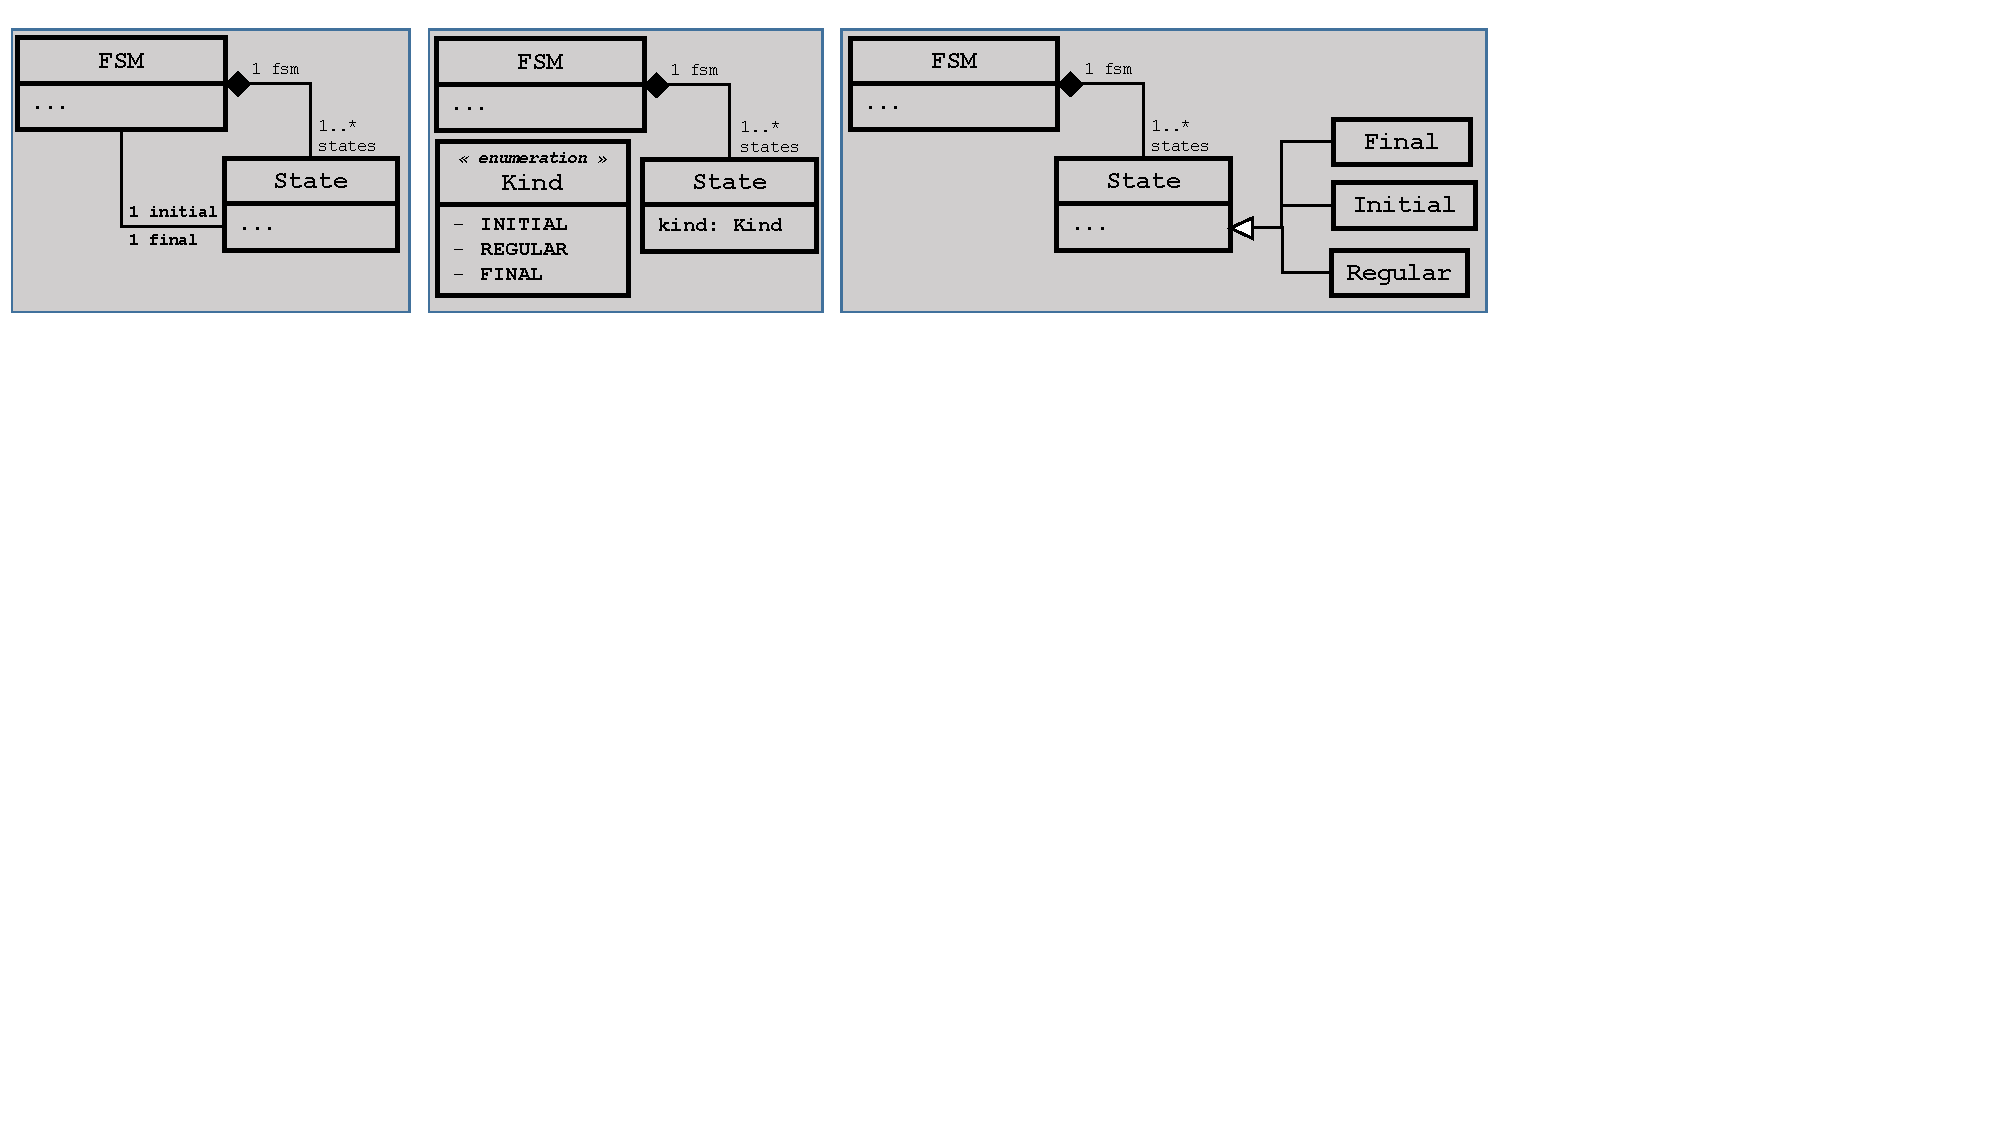
\includegraphics[width=\columnwidth,clip, trim=0cm 13.8cm 8.3cm 0.2cm]{FSM-Initial}%
   \caption{Modelling a \textsf{State} in \textsf{FSM}: with explicit references
   \texttt{initial} and \texttt{final} (left); with a distinguishing property 
   \texttt{kind} (middle); and with inheritance (right).}%
   \label{fig:FSM-Initial}%
   \Description[Different ways of modelling \textsf{FSM}'s \textsf{State}s.]{%
   A \textsf{State} is modelled with explicit references, with a distinguishing 
   property in \textsf{State} specifying, with an enumeration, the different 
   \textsf{kind}s, and with inheritance.}
\end{figure}

\begin{description}
   \item[CS.1. Providing \emph{simple} visualisation of data struc\-tures.]
   Pro\-vi\-ding configurable representations for common data structures such as
   (multi-column) tables, graphs, sets and lists present the benefit of rapidly
   presenting information from a model. This ability should rely on queries to
   identify, and eventually modify, the elements of the model used for ``populating''
   such structures. 

	\item[CS.2. Providing \emph{complex} rendering patterns.]
   Consider the (partial) meta\-models in \autoref{fig:FSM-Initial} that
   specify the \emph{initial} \textsf{State} in four different ways: by referencing
   to the appropriate \textsf{State} among those available, by characterising each \textsf{State} with
   a property \textsf{kind}, or by using type inheritance. Many tools would only
   support the latter, because they essentially only allow to 
   associate various icons to classes. This approach is too simplistic and forces
   metamodel designers to tweak their metamodels towards MA, introducing yet another
   metamodel specialisation (as it is already the case for model editing and
   model analysis, among others). Complex rendering patterns should allow to freely
   associate visual counterparts to various combinations and values of metamodel
   elements.
   
   \item[CS.3. Integrating ``insideness'' \emph{natively}] We call \emph{insideness}
   the visual equivalent of \emph{containment} in metamodelling, i.e. the ability
   to uniquely put elements \emph{inside} inside a container so that elements 
   inside disappear along with the container's removal. This feature presents two
   advantages. First, it would allow to natively handle common situations like 
   including text inside a shape (e.g. displaying a \textsf{State}'s name within
   the circle for an \textsf{FSM}) and then treat them in an universal manner. 
   Second, if the feature is customisable, it would enforce a natural semantics
   graphically with an expected behaviour. 
   
   \item[CS.4. Providing ``snapping'' capabilities] Snapping helps precise\-ly arrange
   graphical elements by ``gluing'' them to a specific target, e.g. a canva's
   boundary, a grid, or points on objects. 
      
   \item[CS.6. Supporting animations natively.] Having at disposal a \DSL
   for defining CSs brings the ability to \emph{visually} render metamodels, but
   does not guarantee the ability to perform animation. For that, the \DSL should
   natively support the fast update of visual features that compose the CS (e.g.,
   the position, size, color, type of line for an \textsf{FSM}'s 
   \textsf{Transition}).      
\end{description}


